% Modelo de slides para projetos de disciplinas do Abel
\documentclass[10pt]{beamer}

\usetheme[progressbar=frametitle]{metropolis}
\usepackage{appendixnumberbeamer}
\usepackage[numbers,sort&compress]{natbib}
\bibliographystyle{plainnat}

\usepackage{booktabs}
\usepackage[scale=2]{ccicons}

\usepackage{xspace}
\newcommand{\themename}{\textbf{\textsc{metropolis}}\xspace}

\title{Finite-Sample Properties of OLS}
% \subtitle{Subtítulo}
% \date{\today}
\date{}
\author{\textbf{Laura Malkhasyan, Aiwei Huang,  Madhurima Chandra}}
\institute{\textbf{University of Bonn}}
% \titlegraphic{\hfill\includegraphics[height=1,5 cm]{logo.pdf}}

\begin{document}

\maketitle

\begin{frame}{Outline}
  \setbeamertemplate{section in toc}[sections numbered]
  \tableofcontents[hideallsubsections]
\end{frame}

\section {Lemma 3.1.1: \\Orthogonal Projection matrices}

\begin{frame}[fragile]{Projection matrices}
\begin{itemize}
\item The (OLS) fitted value: $\hat{\textbf{y}}_i=\mathbf{x}_i\mathbf{b}$\\
In matrix notation: $\hat{\mathbf{y}}=\mathbf{X}\mathbf{b}$   →   $\hat{\mathbf{y}}=\mathbf{X}(\mathbf{X}'\mathbf{X})^{-1}\mathbf{X}'\mathbf{y} = \mathbf{P}\mathbf{y}$\\
Where the (OLS) estimator: $\mathbf{b}=(\mathbf{X}'\mathbf{X})^{-1}\mathbf{X}'\mathbf{y}$
\bigskip
\item The (OLS) residual: $\mathbf{\hat{\boldsymbol{\varepsilon_i}}=y_i-\hat{y}_i}$\\
    In matrix notation:
    {$\hat{\boldsymbol{\varepsilon}} = \mathbf{y}-\hat{\mathbf{y}} = \left(\mathbf{I}_n-\mathbf{X}(\mathbf{X}'\mathbf{X})^{-1}\mathbf{X}'\right)\mathbf{y} = \mathbf{M}\mathbf{y}$}
\end{itemize}
\end{frame}

\begin{frame}[fragile]{Projection matrices}
\item  $\mathbf{P}=\mathbf{X}(\mathbf{X}'\mathbf{X})^{-1}\mathbf{X}'$ is called orthogonal projection matrix  →  projects any vector into the column space spanned by $\mathbf{X}$\\
\item 
$\mathbf{M}=\mathbf{I}_n-\mathbf{X}(\mathbf{X}'\mathbf{X})^{-1}\mathbf{X}'$ is the associated orthogonal projection matrix →  projects any vector into space orthogonal to span of $\mathbf{X}$ 
\end{frame}

\begin{frame}[fragile]{Properties of projection matrices}
\item\textbf{ Lemma 3.1.1 (Orthogonal Projection matrices)}\\
For $\mathbf{P}=\mathbf{X}(\mathbf{X}'\mathbf{X})^{-1}\mathbf{X}'$ and
$\mathbf{M}=\mathbf{I}_n-\mathbf{P}$ , where $\mathbf{X}$ is of full rank:

\begin{enumerate}
\item $\mathbf{P}$ and $\mathbf{M}$ are symmetric and idempotent:
\begin{itemize}
\item $\mathbf{P}=\mathbf{P}'$   and  $\mathbf{M}=\mathbf{M}'$

\item $\mathbf{P}\mathbf{P}=\mathbf{P}\quad\text{and}\quad \mathbf{M}\mathbf{M}=\mathbf{M}$
\end{itemize}
\bigskip
\item $\mathbf{X}'\mathbf{P}=\mathbf{X}',\quad \mathbf{X}'\mathbf{M}=\mathbf{0},\quad\text{ and }\quad \mathbf{P}\mathbf{M}=\mathbf{0}$
\end{enumerate}
\end{frame}

\begin{frame}{Proof}
Can show these properties directly from the definitions of $\mathbf{P}$ and $\mathbf{M}$.\
\begin{enumerate}
\item 
\begin{itemize}
\item $\mathbf{P}'=(\mathbf{X}(\mathbf{X}'\mathbf{X})^{-1}\mathbf{X}')'=\mathbf{X}(\mathbf{X}'\mathbf{X})^{-1}\mathbf{X}'=\mathbf{P}$ \\
$\mathbf{M}'=\mathbf{I}_n-\mathbf{P}'=\mathbf{M}$ 


\item $\mathbf{P}\mathbf{P}=\mathbf{X}(\mathbf{X}'\mathbf{X})^{-1}\mathbf{X}'\mathbf{X}(\mathbf{X}'\mathbf{X})^{-1}\mathbf{X}'=\mathbf{X}(\mathbf{X}'\mathbf{X})^{-1}\mathbf{X}'=\mathbf{P}$\\

$\mathbf{M}\mathbf{M}=(\mathbf{I}_n-\mathbf{P})(\mathbf{I}_n-\mathbf{P})=\mathbf{I}_n-\mathbf{P}=\mathbf{M}$

\end{itemize}

\bigskip

\item
\begin{itemize}
\item $\mathbf{X}'\mathbf{P}=\mathbf{X}'\mathbf{X}(\mathbf{X}'\mathbf{X})^{-1}\mathbf{X}'=\mathbf{X}'$
\item $\mathbf{X}'\mathbf{M}=\mathbf{X}'(\mathbf{I}_n-\mathbf{P})=\mathbf{X}'-\mathbf{X}'\mathbf{P}=\mathbf{0}$
\item $\mathbf{P}\mathbf{M}=\mathbf{P}(\mathbf{I}_n-\mathbf{P})=\mathbf{0}$

\end{itemize}
\end{enumerate}
\end{frame}


\section {Proposition 3.1.2: \\OLS residuals}

\begin{frame}[fragile]{OLS residuals}
  The n-vector \boldmath$y-X\beta$ is called residual, with \boldmath$\beta$ allowed to vary arbitrarily.\\
  The \textbf{OLS residual} is the one that orthogonal to the column space spanned by \boldmath$X$ or the subspace \boldmath$S(X_{1}, X_{2}, \dots, X_{K})$.
\end{frame}

\begin{frame}[fragile]{OLS residuals}
        \centering
        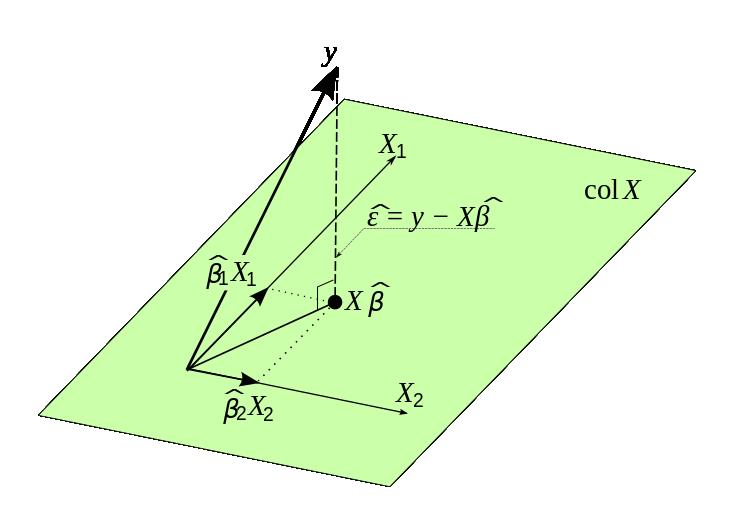
\includegraphics[width=\textwidth]{OLS.jpg}
        \caption{OLS geometric interpretation.}
\end{frame}

\begin{frame}[fragile]{Theorem and Proof}
  \textbf{Proposition 3.1.2 (OLS residuals)}\\
  For the OLS residuals and the OLS fitted values it holds that\\
\begin{align*}
    \mathbf{X}'\hat{\boldsymbol{\varepsilon}} = \mathbf{0}, \quad\text{and}\\
    \mathbf{y}'\mathbf{y} = \hat{\mathbf{y}}'\hat{\mathbf{y}}+\hat{\boldsymbol{\varepsilon}}'\hat{\boldsymbol{\varepsilon}}.
\end{align*}
\end{frame}

\begin{frame}[fragile]{Theorem and Proof}
\textbf{Proof.}\\
\begin{align*}
  \mathbf{X}'\hat{\boldsymbol{\varepsilon}} 
   &= \mathbf{X}'\mathbf{M}\mathbf{y}\quad\text{(By Def. of $\mathbf{M}$)}\\
   &= \mathbf{0}\mathbf{y}\quad\text{(By Lemma 3.1.1 part (ii))}\\
   &= \underset{(K\times 1)}{\mathbf{0}}
\end{align*}  

\begin{align*}
  \mathbf{y}'\mathbf{y} &= (\mathbf{P}\mathbf{y}+\mathbf{M}\mathbf{y})'(\mathbf{P}\mathbf{y}+\mathbf{M}\mathbf{y})\quad\text{(By Def.~of $\mathbf{P}$ and $\mathbf{M}$)}\\
   &= (\mathbf{y}'\mathbf{P}'+\mathbf{y}'\mathbf{M}')(\mathbf{P}\mathbf{y}+\mathbf{M}\mathbf{y})\\
   &= \mathbf{y}'\mathbf{P}'\mathbf{P}\mathbf{y}+\mathbf{y}'\mathbf{M}'\mathbf{M}\mathbf{y}+\mathbf{0}\quad\text{(By Lemma 3.1.1 part (ii))}\\
   &= \hat{\mathbf{y}}'\hat{\mathbf{y}}+\hat{\boldsymbol{\varepsilon}}'\hat{\boldsymbol{\varepsilon}}
\end{align*}
\end{frame}

\begin{frame}[fragile]{Unbiased Variance Estimator}
\textbf{Def.}\\
\begin{align*}
  s^2 = \frac{1}{n-K}\sum_{i=1}^n\hat{\varepsilon_i^2}
\end{align*}
  Why $n-K$ degrees of freedom ?\\
  $\hat{\varepsilon_i^2}$ loses $K$ degrees of freedom because it has to satisfy the $K$ linear restrictions
  ($\mathbf{X}'\hat{\boldsymbol{\varepsilon}} &= \mathbf{0}$).
\end{frame}


\section {Proposition 3.1.3: \\Variance Decomposition}

\begin{frame}{Variance Decomposition}
Total sample variance of dependent variable (for a linear model with intercept) can be decomposed into variance explained by the regressors and variance explained by other factors unaccounted for in the model:
\begin{align*}
  \underset{\text{total variance}}{\sum_{i=1}^n\left(y_i-\bar{y}\right)^2} = \underset{\text{explained variance}}{\sum_{i=1}^n\left(\hat{y}_i-\bar{\hat{y}}\right)^2}+\underset{\text{unexplained variance}}{\sum_{i=1}^n\hat{\varepsilon_i}^2 \,\,}
\end{align*}
\end{frame}



\begin{frame}{Variance Decomposition: Proof}
From Proposition 3.1.2, we know that
    $\sum_{i=1}^n\hat{\varepsilon_i} = 0$, for regressions with intercept. \\Hence, from $y_i=\hat{y}_i+\hat{\varepsilon_i}$
    it follows that \begin{align*}
      \frac{1}{n}\sum_{i=1}^n y_i &= \frac{1}{n}\sum_{i=1}^n \hat{y}_i+\frac{1}{n}\sum_{i=1}^n \hat{\varepsilon_i} \\
      \bar{y} &= \bar{\hat{y}}_i+0 \end{align*}
\end{frame}

\begin{frame}{Variance Decomposition: Proof (Contd.)}
From Proposition 3.1.2, we know: \begin{align*}
\mathbf{y}'\mathbf{y} &= \hat{\mathbf{y}}'\hat{\mathbf{y}}+\hat{\boldsymbol{\varepsilon}}'\hat{\boldsymbol{\varepsilon}} \\
       \mathbf{y}'\mathbf{y} -n\bar{y}^2 &= \hat{\mathbf{y}}'\hat{\mathbf{y}}-n\bar{y}^2+\hat{\boldsymbol{\varepsilon}}'\hat{\boldsymbol{\varepsilon}} \\
       \mathbf{y}'\mathbf{y}-n\bar{y}^2 &= \hat{\mathbf{y}}'\hat{\mathbf{y}}-n\bar{\hat{y}}^2+\hat{\boldsymbol{\varepsilon}}'
       \hat{\boldsymbol{\varepsilon}}\quad\text{(since $\bar{y} &= \bar{\hat{y}}_i$)} \\
       \sum_{i=1}^n y_i^2-n\bar{y}^2 &= \sum_{i=1}^n\hat{y}_i^2-n\bar{\hat{y}}^2+\sum_{i=1}^n\hat{\varepsilon}_i^2 \\
       \sum_{i=1}^n (y_i-\bar{y})^2 &= \sum_{i=1}^n
       (\hat{y}_i-\bar{\hat{y}})^2+\sum_{i=1}^n \hat{\varepsilon}_i^2
\end{align*}
\end{frame}

\begin{frame}{Coefficient of Determination $R^2$}
\begin{align*}
  R^2=\frac{\sum_{i=1}^n\left(\hat{y}_i-\bar{\hat{y}}\right)^2}{\sum_{i=1}^n\left(y_i-\bar{y}\right)^2}\;=\;1-\frac{\sum_{i=1}^n\hat{u}_i^2}{\sum_{i=1}^n\left(y_i-\bar{y}\right)^2}
\end{align*}
\begin{itemize} \item Ratio of 'explained' variance to the 'total' variance of dependent variable.
\item Larger the proportion of explained variance, better is the fit of the model.
\item $0\leq R^2\leq 1$.
\item Disadvantage of using $R^2$ as a measure of goodness-of-fit.
\end{itemize}
\end{frame}

\end{document}
